\documentclass{article} % For LaTeX2e
\usepackage{nips14submit_e,times}
\usepackage{amsmath}
\usepackage{fancyvrb}
\usepackage{hyperref}
\usepackage{url}
\usepackage{graphicx}
%\documentstyle[nips14submit_09,times,art10]{article} % For LaTeX 2.09


\title{A4 homework submission \\ David Halpern \\ Deep Learning 2015, Spring}


\author{
David Halpern\\
Department of Psychology\\
New York University\\
\texttt{david.halpern@nyu.edu} \\
}

\newcommand{\fix}{\marginpar{FIX}}
\newcommand{\new}{\marginpar{NEW}}

\nipsfinalcopy % camera-ready version

\begin{document}


\maketitle


\section{Questions}

\subsection{Q2}

i = i\\
$\text{prev\_c} = c_{t-1}^l$\\
$\text{pre\_h} = h_{t-1}^l$

\subsection{Q3}
Returns a rolled version of the core RNN module with parameters initialized uniformly within an interval.

\subsection{Q4}
model.s is the trained of the sequence. model.ds is the gradients of the model for the backward pass. model.start$\_$s is the final hidden states of the current minibatch and gets reset when the sequence ends

\subsection{Q5}
Clipped at params.max$\_$grad$\_$norm (shrink factor?)

\subsection{Q6}
Batch SGD

\subsection{Q7}
Since the prediction was essentailly outside the model and the nLL criterion was computed before the prediction, the prediction should have no impact on the gradient so the gradient is a large table of 0s.

\section{Model}
\subsection{Architecture}
The basic model used was very similar to the one used by Zaremba (2014). The model uses a Long Short-Term Memory (LSTM) cell as the basic neural unit (see Figure 1). 
\begin{figure}
	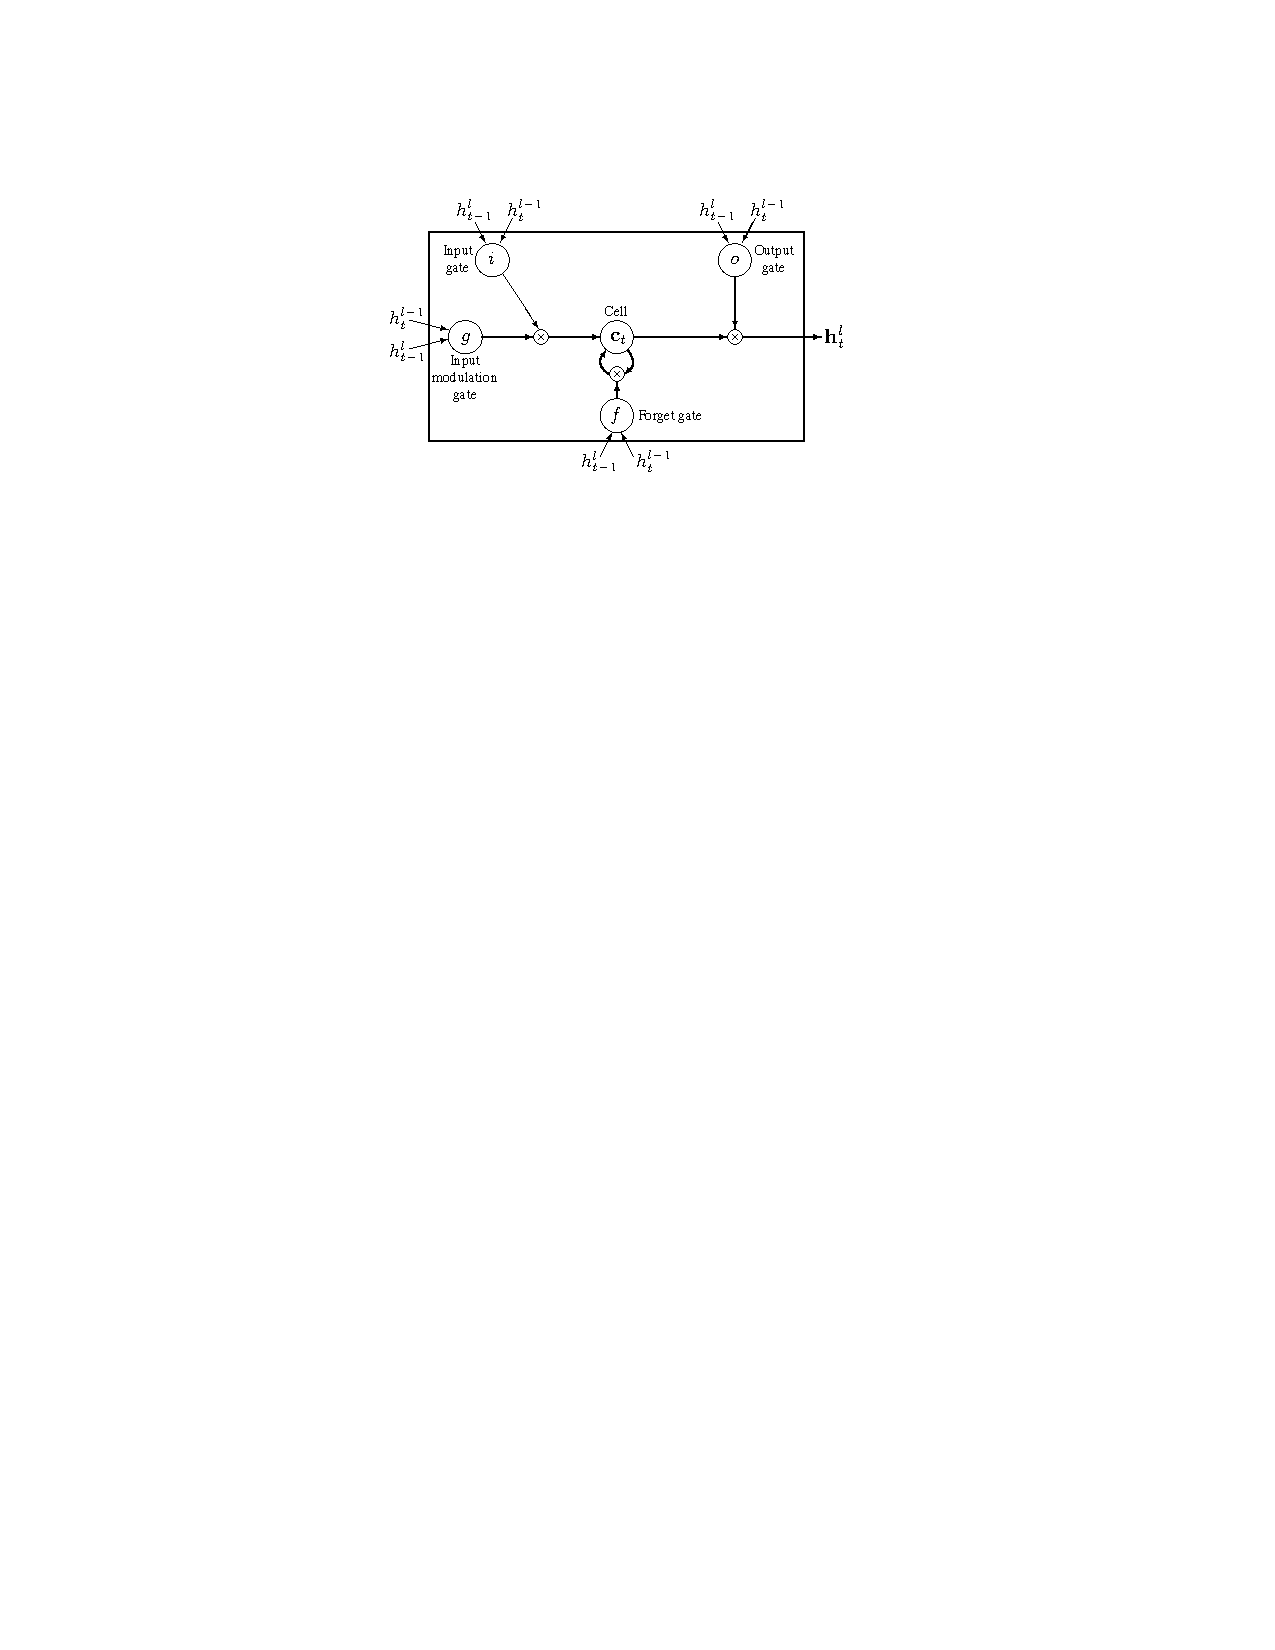
\includegraphics[width=\textwidth]{LSTMcell}
        \label{fig1}
        \caption{Example LSTM cell}
\end{figure}
The LSTM proceeds by computing the equations in Figure 2. The cell in a particular layer takes as input $h_t^{l-1}$, the state of the previous layer at time $t$, and $h_{t-1}^l$, the state of the current layer at the previous time step.
\begin{figure}
	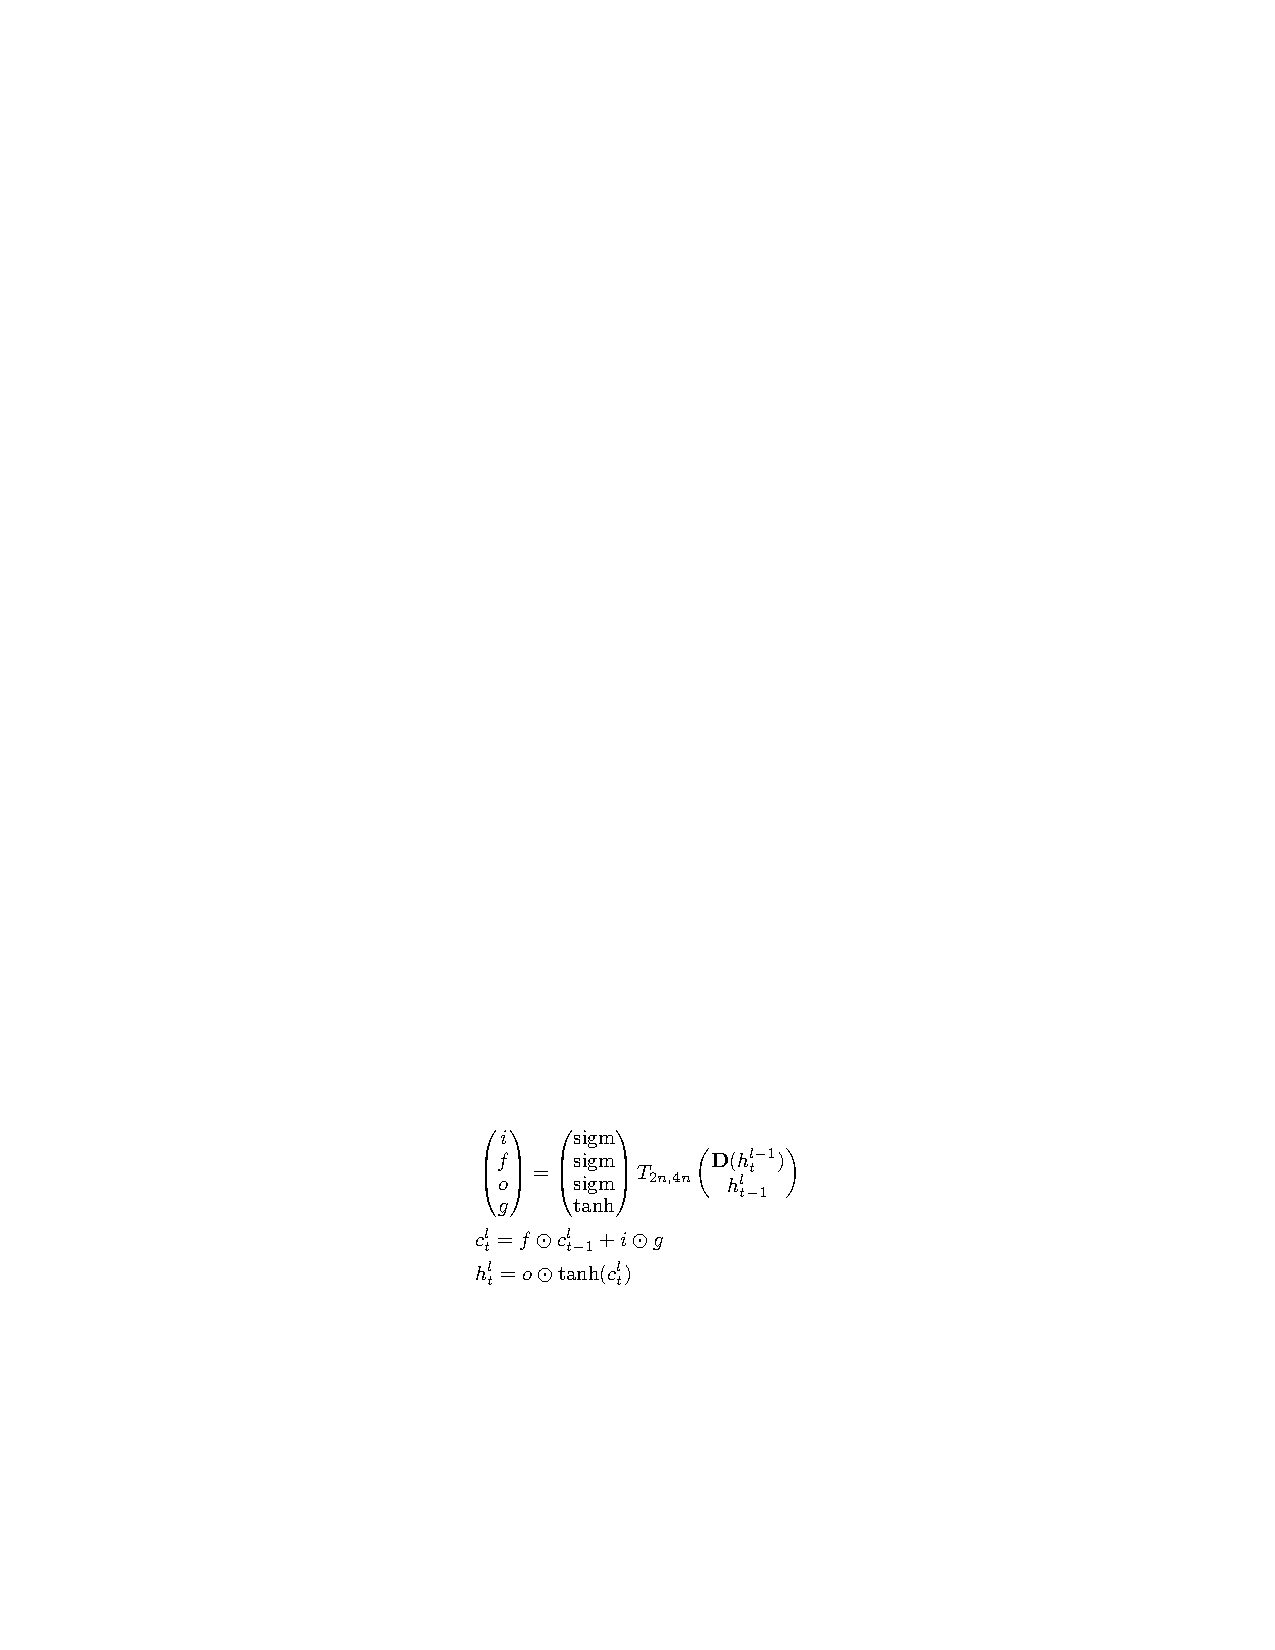
\includegraphics[width=\textwidth]{LSTMeqs}
        \label{fig2}
        \caption{Example LSTM cell}
\end{figure}
These cells are combined into a standard recurrent neural network with two layers (Figure 3).
\begin{figure}
	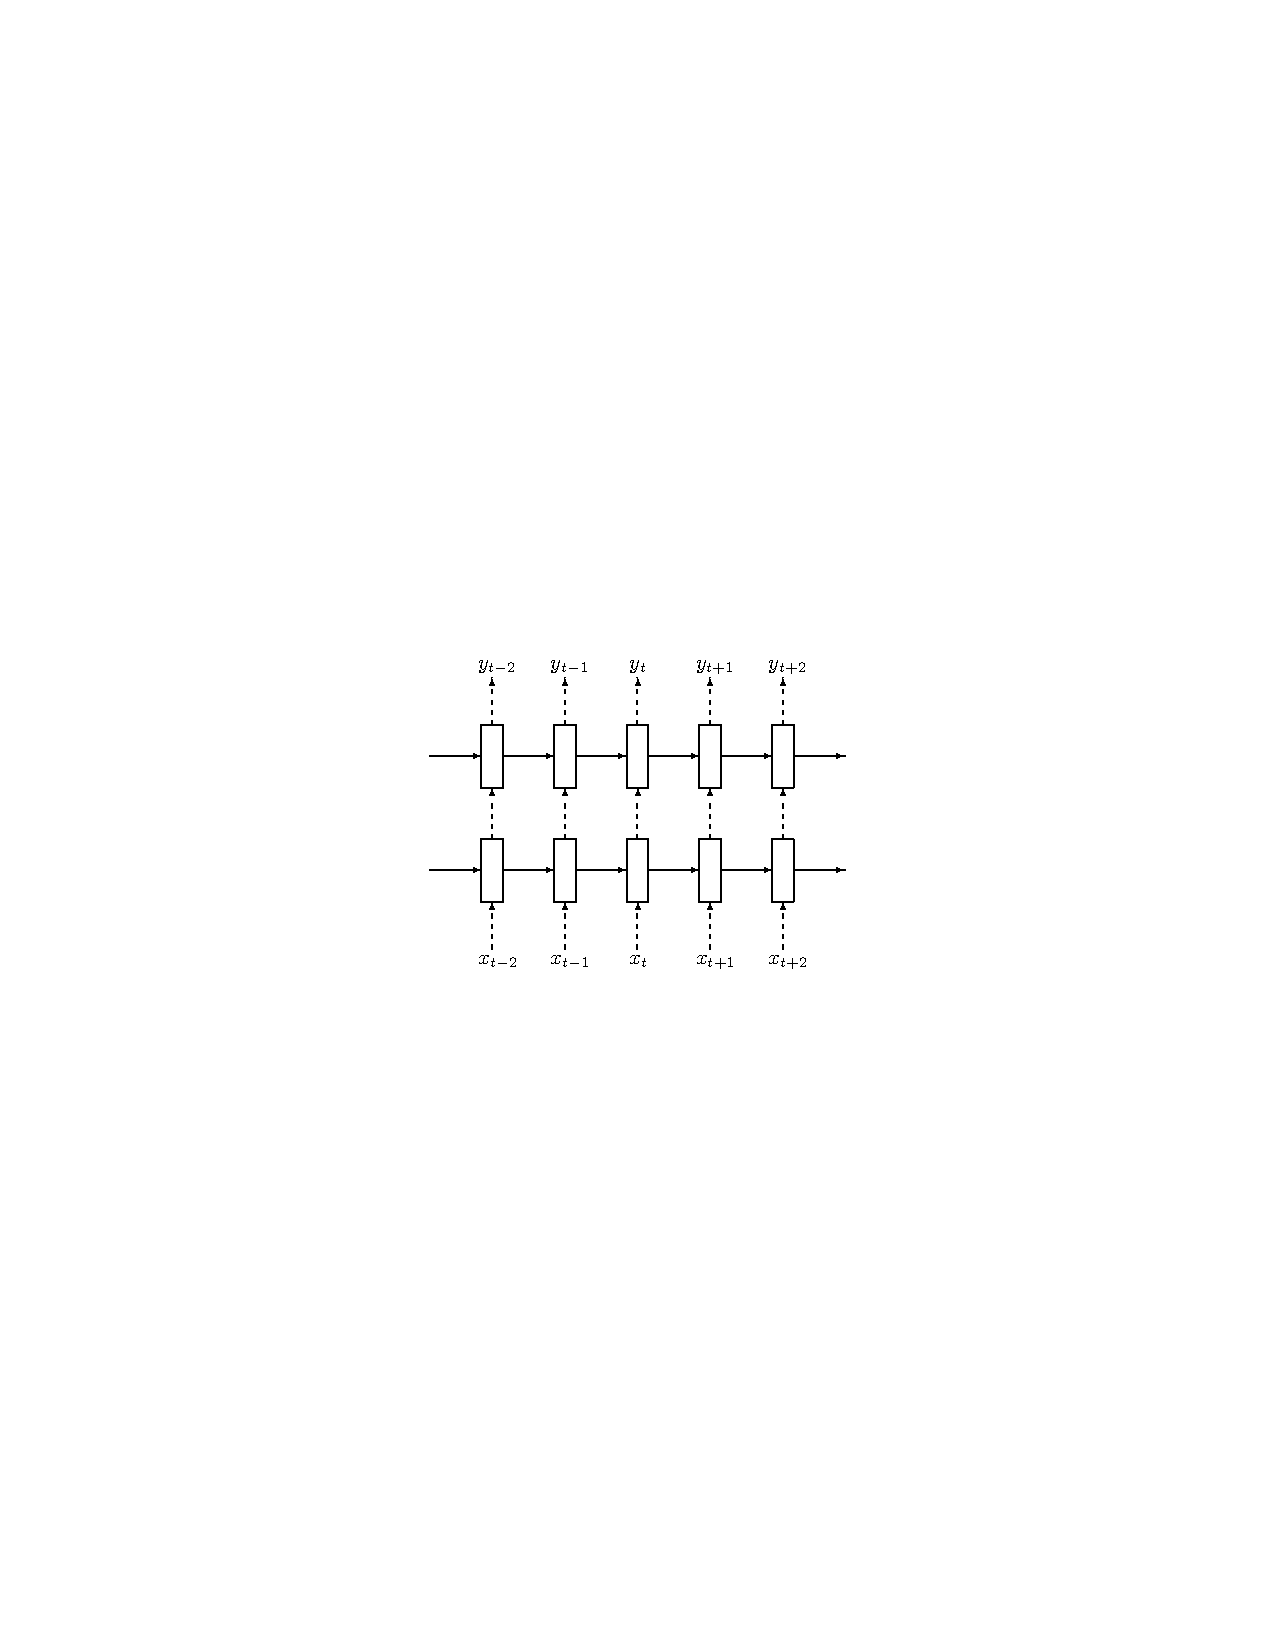
\includegraphics[width=\textwidth]{MultilayerRNN}
        \label{fig2}
        \caption{Example RNN. $x_t$ is the previous character and $y_t$ is the next character to be predicted}
\end{figure}
In order to be read by the network, words and characters were transformed into a sparse vector representation with each column representing a word in the vocabulary of the model. The Penn Treebank dataset included 10000 words in it's vocabulary and 50 characters. The model was unrolled to a sequence length of 20.

\subsection{Training}
The model was trained using mini-batches of size 20, a learning weight of 1, a gradient clip of 5 and no dropout. Parameters were initialized uniformly on [-.1, 1]. After the fourth epoch, learning rates decayed by half every epoch. The model was run for 13 epochs. The Penn Treebank contains 929k words in its training set, 73k words in it's validation set and 82k words in its test set. 

\section{Experiments}
\subsection{1} 
In this experiment, I attempted to increase the number of nodes in the rnn from 200 to 400, under the assumption that more nodes would allow for more discriminable states of the network. Having more states also increased the effectiveness of dropout since there were still more nodes turned on even while training so I used a dropout rate of .2. Dropout and more nodes allow for relaxing the gradient clipping from 5 to 7 since there is more regularization. This (theoretically) allows for more flexibility in learning the parameters in the larger network. The model was also unrolled to a length of 50 under the assumption that memory could be stored longer in the bigger network. However, in order to speed up the training scheme, I used a batch size of 50. It is possible that this had a negative effect on parameter learning and in the end perplexity of this model bottomed out at 367.211 after 13 epochs. 
Network parameters:	
\begin{Verbatim}
{
  max_grad_norm : 7
  seq_length : 50
  batch_size : 50
  lr : 1
  max_max_epoch : 13
  rnn_size : 400
  init_weight : 0.1
  decay : 2
  dropout : 0.2
  layers : 2
  vocab_size : 50
  max_epoch : 4
}
\end{Verbatim}

\subsection{2}
In this model, I simply tried increasing the number of layers. I used a small amount of dropout here to regularize the gradients which could explode even more in the larger network. Again to speed up training, I used a larger batch size which likely had a negative impact and this model got to a validation perplexity of 425.576 after 13 epochs.
\begin{Verbatim}
Network parameters:	
{
  max_grad_norm : 5
  seq_length : 50
  batch_size : 50
  lr : 1
  max_max_epoch : 13
  rnn_size : 200)
  init_weight : 0.1
  decay : 2
  dropout : 0.2
  layers : 3
  vocab_size : 50
  max_epoch : 4
}
\end{Verbatim}

\subsubsection*{References}

\small{
[1] Zaremba, W., Sutskever, I., \& Vinyals, O. (2014). Recurrent Neural Network Regularization. Arxiv, http://arxiv.org/pdf/1409.2329v4.pdf
}


\end{document}
